In authentication, when the user successfully logs in using their credentials, a JSON Web Token will be returned.
Since tokens are credentials, great care must be taken to prevent security issues.
In general, you should not keep tokens longer than required.
You also should not store sensitive session data in browser storage due to lack of security.
Whenever the user wants to access a protected route or resource, the user agent should send the JWT,
typically in the Authorization header using the Bearer schema.
The content of the header should look like the following:
\begin{spverbatim}

    Authorization: Bearer <token>

\end{spverbatim}
This can be, in certain cases, a stateless authorization mechanism.
The server's protected routes will check for a valid JWT in the Authorization header, and if it's present,
the user will be allowed to access protected resources.
If the JWT contains the necessary data, the need to query the database for certain operations may be reduced,
though this may not always be the case.
If the token is sent in the Authorization header, Cross-Origin Resource Sharing (CORS) won't be an issue
as it doesn't use cookies.
Generally, the workflow is as follows
% old
\begin{enumerate}
    \item User provides credentials in order to authenticate to the system.
    \item Server verifies user's authentication, fetches the login and password in database.
    \item If authentication is successful, server creates session then writes this session to the database,
    see table session in [REFERENCE\_DATABASE\_SCHEMA].
    \item Server generates a pair of access token (JWT) and refresh token (GUID).
    \item Server sends to client access token and refresh token.
    \item Client saves the pair of access and refresh tokens.
    \item User requests resource using received token passed to the request header.
    \item The server check user's claims and proceeds or declines request.
\end{enumerate}

The eighth point is the authorization.
As a result, token stored on the client and used when it is necessary to authorize the requests.
When a hacker tries to replace the data in the header or payload the token will become invalid,
therefore the signature will not match the original values.
So, the hacker hasn't any possibility to generate a new signature since that encryption secret key stored on the server.
Access token (JWT) is used for request authorization and for storing the additional information about user like identifier,
display name and others.
Refresh Token (GUID) issued by server based on successful authentication results and used for get new access/refresh
token pair.
Also, it is worth to add a few basic rules about JWT secure usage [\cite{RDegges}]
\begin{itemize}
    \item JWT should have a short lifetime, since it cannot be revoked.
    \item JWT should be used in a single time, e.g JWT per request.
\end{itemize}
Therefore, we consider access token's lifetime to be 5 minutes and refresh token's 7 days.

For each request client preliminarily checks access token's lifetime.
If access token it expired, client sends request for updating a pair of access/refresh tokens.
For more confidence, we can update tokens a few seconds earlier.
That is, the case when the API receives an expired access token is practically excluded.
However, we are able to consider the case of interception of the request on 401 http response code,
that is unauthorized.
The following diagram demonstrates the process of requesting the resource

\begin{figure}[H]
    \centering
    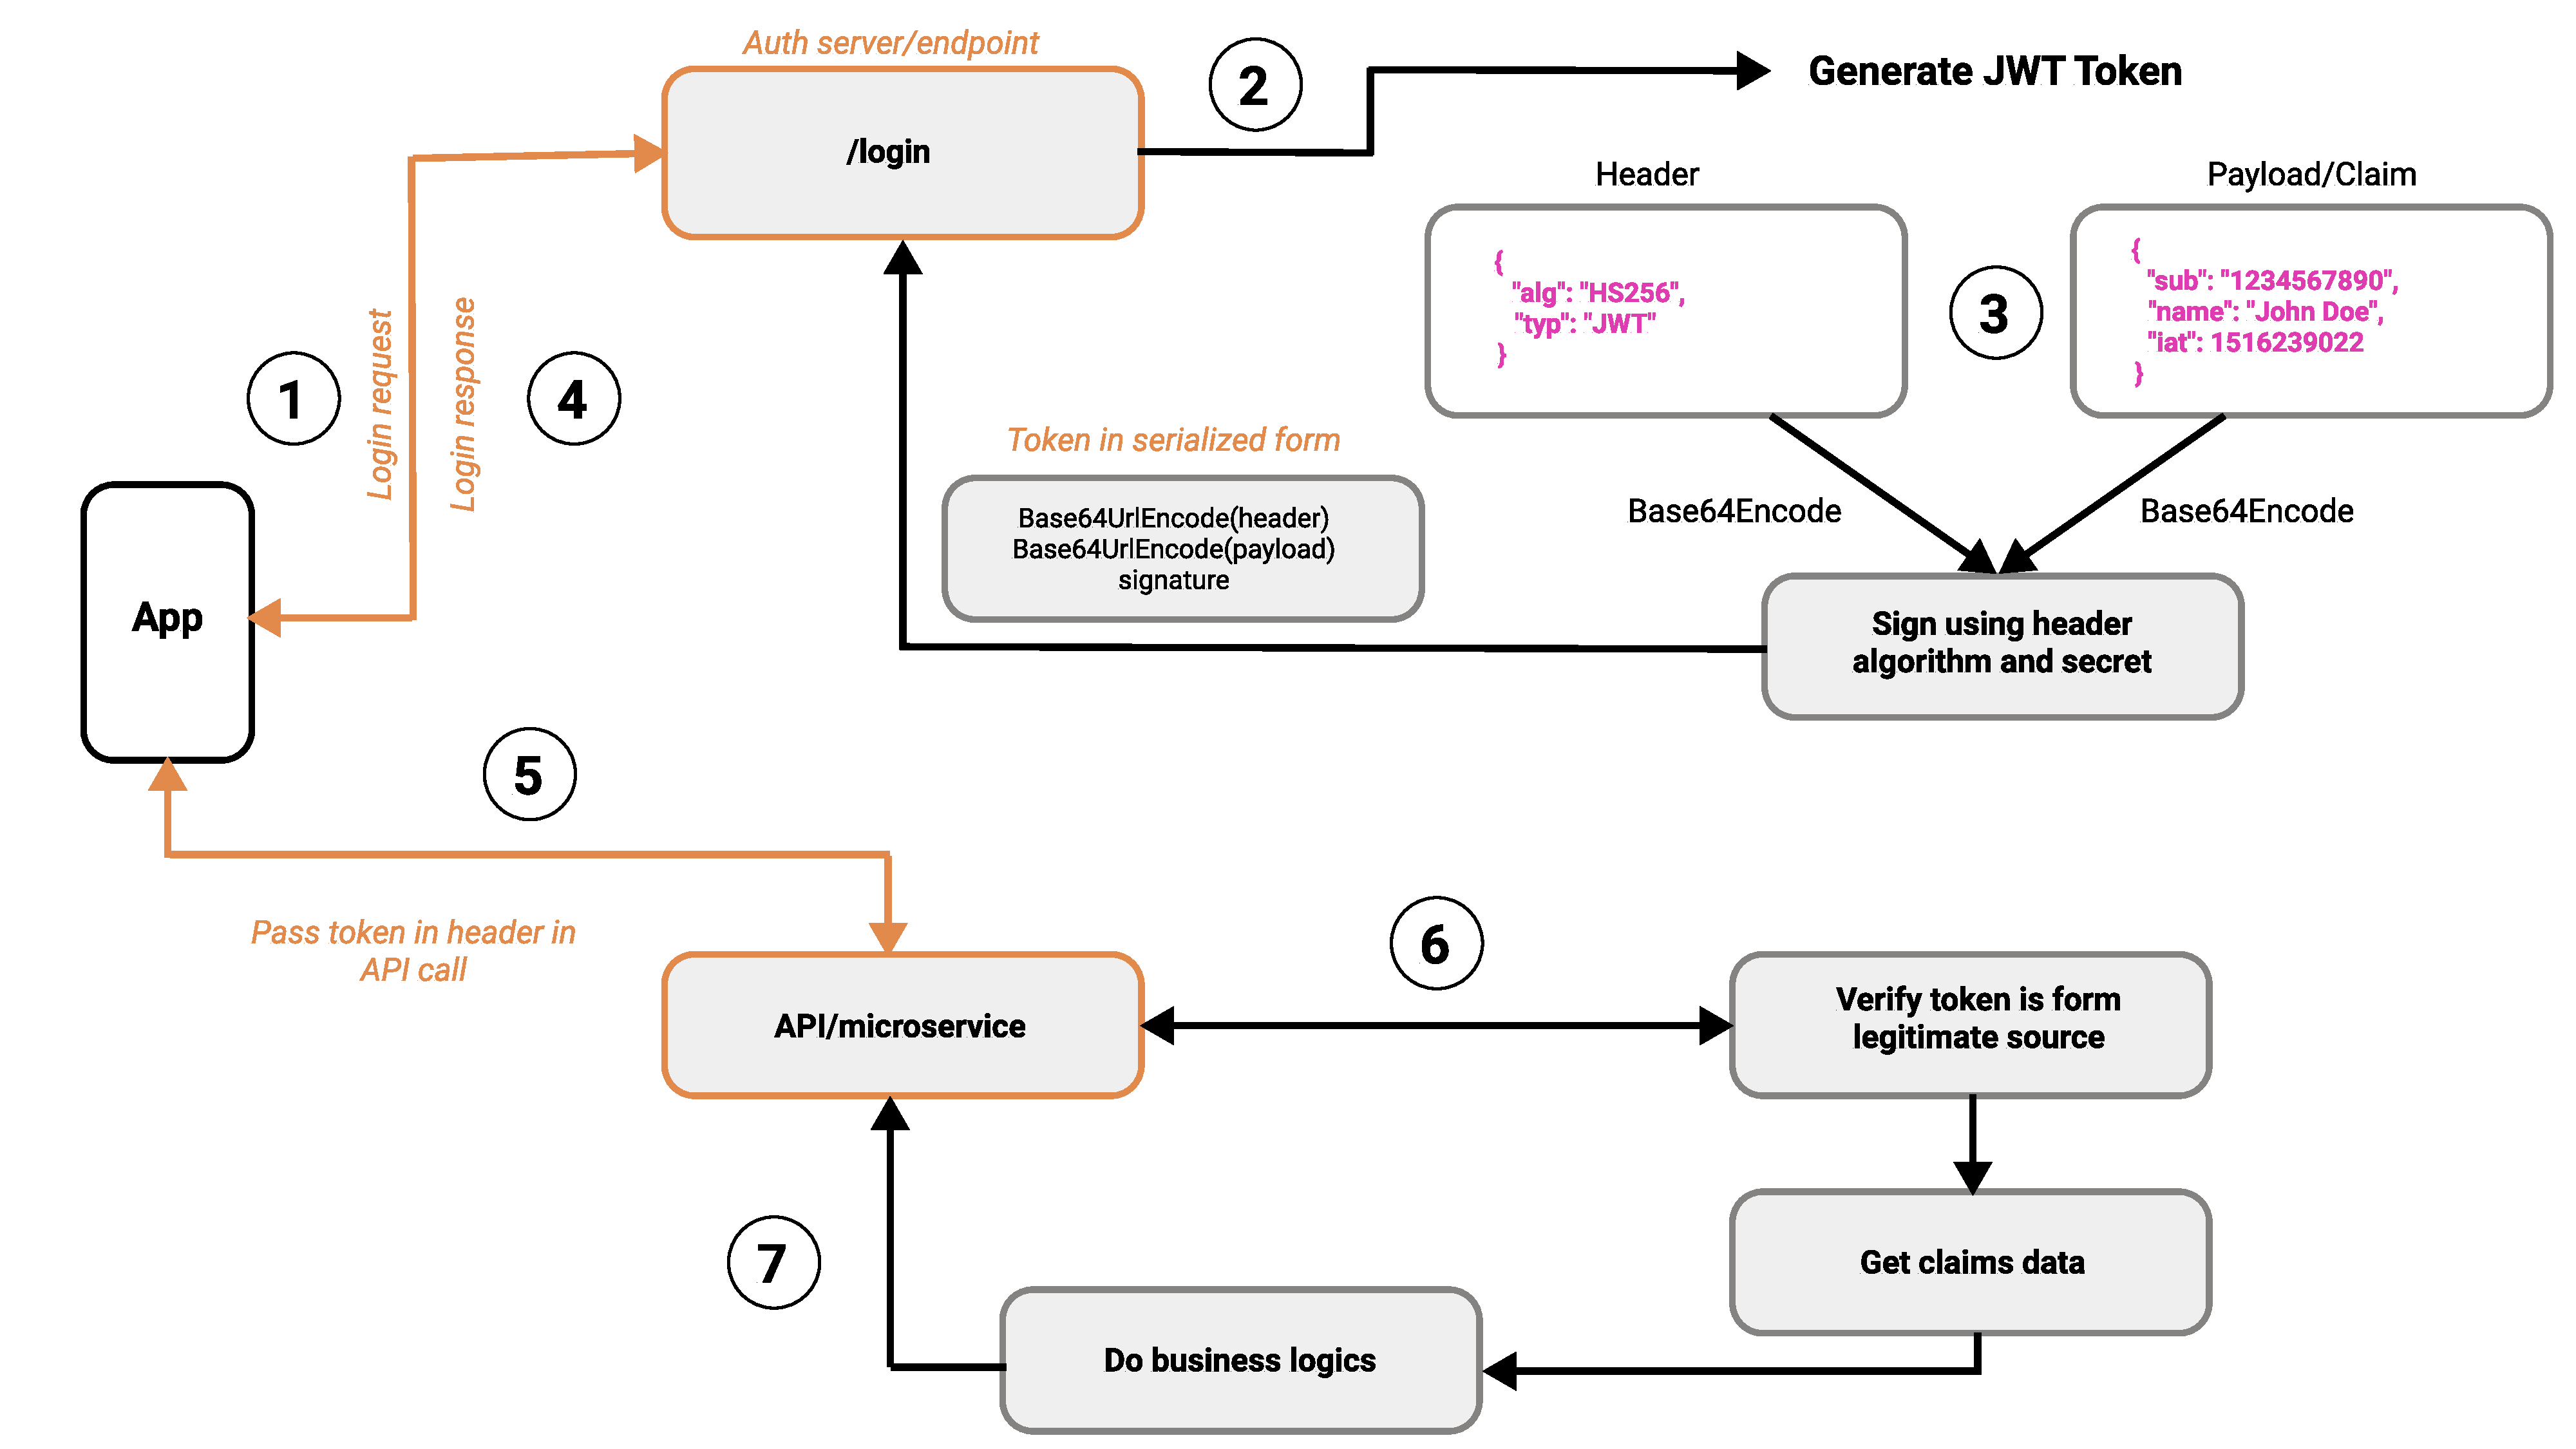
\includegraphics[width=1\textwidth]{Pictures/jwt_auth_scheme.pdf}
    \caption{JWT Authentication concept diagram.}\label{fig:figure3}
\end{figure}

By steps, the process is
\begin{enumerate}
    \item The client app sends request with credentials to the authentication endpoint of an API\@.
    \item On authentication success, the server proceeds to generate a pair of access/refresh tokens,
    otherwise returns 409Conflict Http code response to the client.
    \item Server generates a pair of access/refresh tokens
    \begin{itemize}
        \item API fetches user data and claims.
        \item Server creates new session instance in database.
        \item Header base64 encoded.
        \item Payload, or user claims are base64 encoded.
        \item Encoded header and payload signed using the algorithm in the header.
    \end{itemize}
    \item Access token in serialized form and refresh token (GUID) returned in response to the client.
    \item The client queries the API providing access token in request header.
    \item API validates the token claims
    \begin{itemize}
        \item On success, goes to step 7.
        \item On 401Unauthorized Http response code, goes to step 1.
    \end{itemize}
    \item API returns response to the client according to app's business logic.
\end{enumerate}